\documentclass[11pt]{article}
\usepackage[utf8]{inputenc}
\usepackage[spanish]{babel}
\usepackage{amsmath,amssymb,amsthm}
\usepackage{graphicx}
\usepackage[margin=2.5cm]{geometry}
\usepackage{enumitem}
\title{Semana 6 -- Materia}
\author{Tutorías -- Introducción al Cálculo}
\date{07/09--11/09/2026}
\begin{document}
\maketitle

\section{Concepto de función}

Ya sabemos (de las semanas anteriores) qué es una relación en $\mathbb{R} \times \mathbb{R}$: un
conjunto de pares ordenados. Una \textbf{función} es un tipo particular de relación, en la que cada
elemento del dominio tiene una \emph{única} imagen asociada. Pensemos en la operación ``el cuadrado
de \ldots'', que a cada número real $r$ le asigna $r^2$: esta operación queda determinada por los
pares $(x,y) \in \mathbb{R}\times\mathbb{R}$ tales que $y=x^2$, es decir, por la relación
$\{(x,y)\in\mathbb{R}\times\mathbb{R} : y=x^2\}$. Lo especial de esta relación, a diferencia de una
relación cualquiera, es que para cada $x$ hay exactamente un $y$ asociado. Esta idea se formaliza en
la siguiente definición.

\subsection*{Definición 3.6 (Función)}

$F$ es una función si y sólo si $F$ es una relación y
\[
\forall x \in \text{DOM}\, F \ \exists! \, y \in \text{REC}\, F \ \big( (x,y) \in F \big).
\]

Es decir, $F$ es función cuando todo elemento de su dominio tiene una y sólo una imagen en $F$
(el símbolo $\exists!$ se lee ``existe un único'').

\subsection*{Definición 3.7 (Función de $A$ en $B$)}

Si $A$ y $B$ son conjuntos, entonces $F$ \textbf{es función de $A$ en $B$} si y sólo si $F$ es
función, $\text{DOM}\, F = A$ y $\text{REC}\, F \subseteq B$. En ese caso escribimos $F : A \to B$,
y la única imagen de $x$ por $F$ se denota $y = F(x)$.

Gráficamente, una relación es función si y sólo si toda recta vertical corta a su gráfico en
\textbf{a lo más un punto}: si una recta vertical $x = a$ cortara el gráfico en dos puntos
$(a, y_1)$ y $(a, y_2)$ con $y_1 \neq y_2$, entonces $a$ tendría dos imágenes distintas y $F$ no
sería función.

Finalmente, dos funciones $F$ y $G$ son \textbf{iguales} si y sólo si tienen el mismo dominio y
coinciden en cada punto de él: $\text{DOM}\, F = \text{DOM}\, G$ y
$\forall x \in \text{DOM}\, F \ (F(x) = G(x))$.

\subsection*{Ejemplos}

\textbf{Ejemplo 1.} $F = \{(x,y) \in \mathbb{R}\times\mathbb{R} : x = y^2\}$ \textbf{no} es función:
basta ver que $(1,1) \in F$ y $(1,-1) \in F$, con $1 \neq -1$, es decir, $x=1$ tiene dos imágenes
distintas. (Geométricamente, esta relación es una parábola ``acostada'', a la que una recta
vertical como $x=1$ la corta en dos puntos.)

\textbf{Ejemplo 2.} $F = \{(x,y) \in \mathbb{R}\times\mathbb{R} : y = x^2\}$ sí es función de
$\mathbb{R}$ en $\mathbb{R}$: para cada $x \in \mathbb{R}$ hay un único $y$ que cumple $y = x^2$.
Aquí $\text{DOM}\, F = \mathbb{R}$ y $\text{REC}\, F = \mathbb{R}^+ \cup \{0\}$, pues $x^2 \ge 0$
para todo $x$ y todo real no negativo es cuadrado de algún $x$.

\textbf{Ejemplo 3.} Dado un conjunto $A$, la \textbf{función identidad} sobre $A$ se define como
$\text{ID}_A = \{(x,y) \in A \times A : x = y\}$. Es función, con dominio y recorrido iguales a $A$,
pues cada $x \in A$ se asocia únicamente consigo mismo: $\text{ID}_A(x) = x$.

\textbf{Ejemplo 4.} $F = \{(1,2),(2,2),(3,5)\}$, vista como función de $A=\{1,2,3\}$ en
$\mathbb{R}$, es función: cada elemento de $A$ aparece como primera coordenada exactamente una vez
(que dos elementos distintos, $1$ y $2$, compartan la misma imagen $2$ no es problema; lo que no
puede pasar es que un mismo $x$ tenga dos imágenes distintas). Aquí
$\text{REC}\, F = \{2,5\} \subsetneq \mathbb{R}$.

\section{Gráficos de las funciones reales}

Como toda función es en particular una relación, su gráfico se construye exactamente igual que el
de cualquier relación: ubicamos en el plano todos los pares $(x, F(x))$ con $x \in \text{DOM}\, F$.
La diferencia, de acuerdo a lo visto en la sección anterior, es que el resultado siempre superará el
``test de la recta vertical''. A continuación repasamos los gráficos de algunas funciones reales
básicas.

\subsection*{Ejemplo 1: función lineal}

Graficar $F(x) = -2x+5$, $x \in \mathbb{R}$.

Como función, $F = \{(x,y)\in\mathbb{R}\times\mathbb{R} : y=-2x+5\}$, cuyo gráfico es una recta. Para
dibujarla basta ubicar dos puntos, por ejemplo la intersección con cada eje: si $x=0$, $y=5$, y si
$y=0$, $x=5/2$. Una tabla de valores auxiliar:

\begin{center}
\begin{tabular}{|c|c|c|c|}
\hline
$x$ & $0$ & $5/2$ & $3$ \\
\hline
$F(x)$ & $5$ & $0$ & $-1$ \\
\hline
\end{tabular}
\end{center}

\begin{center}
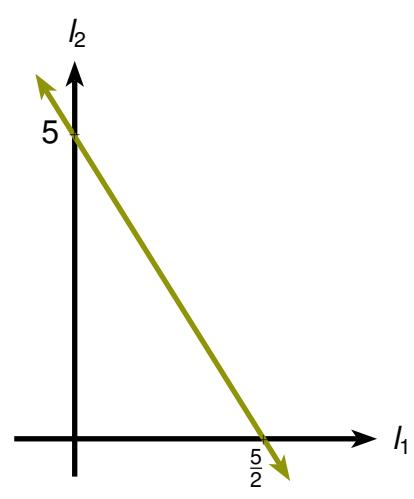
\includegraphics[width=0.55\textwidth]{img/_page_117_Figure_12.jpeg}
\end{center}
Gráfico de $F(x) = -2x+5$, $x \in \mathbb{R}$ (recta que pasa por $(0,5)$ y $(5/2,0)$).

\subsection*{Ejemplo 2: función cuadrática}

Graficar $F(x) = 2x^2 + 6x - 1$.

Completando cuadrados:
\[
2x^2+6x-1 = 2\left(x+\frac{3}{2}\right)^2 - \frac{11}{2},
\]
de donde $y = F(x) \leftrightarrow \left(y+\dfrac{11}{2}\right) = 2\left(x+\dfrac{3}{2}\right)^2$,
que es la ecuación de una parábola con vértice $P\left(-\dfrac{3}{2}, -\dfrac{11}{2}\right)$, que
abre hacia arriba (pues el coeficiente de $x^2$ es positivo) y corta al eje $X$ en los puntos donde
$2\left(x+\frac{3}{2}\right)^2 = \frac{11}{2}$, es decir en
$x = -\dfrac{3}{2} \pm \dfrac{\sqrt{11}}{2}$.

\begin{center}
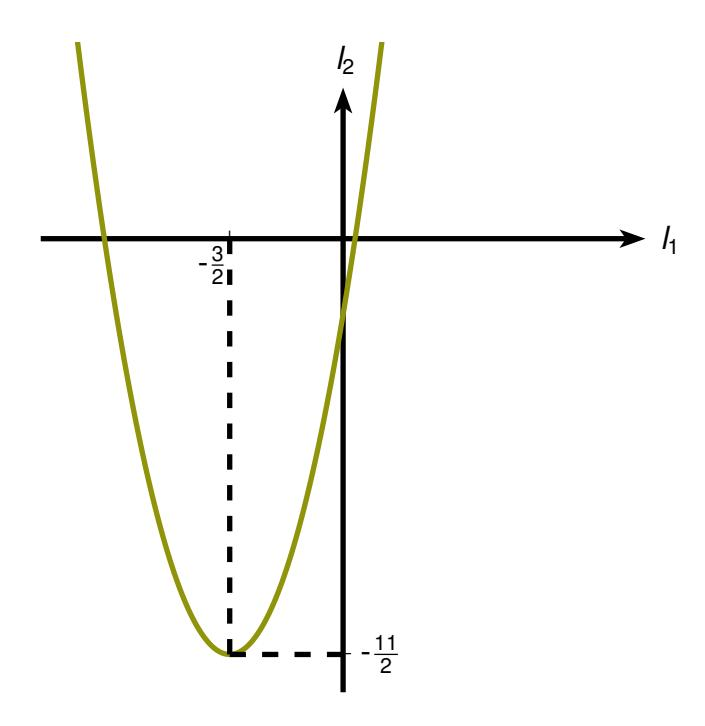
\includegraphics[width=0.5\textwidth]{img/_page_118_Figure_12.jpeg}
\end{center}
Gráfico de $F(x) = 2x^2+6x-1$: parábola con vértice $\left(-\frac{3}{2},-\frac{11}{2}\right)$.

\subsection*{Ejemplo 3: función valor absoluto}

Graficar $f(x) = |x|$.

Por la Definición 2.7, si $x \ge 0$ entonces $f(x) = x$ (recta $y=x$) y si $x<0$ entonces
$f(x) = -x$ (recta $y=-x$). El gráfico resulta ser la unión de dos semirrectas que forman una
``V'':

\begin{center}
\begin{tabular}{|c|c|c|c|c|c|}
\hline
$x$ & $-2$ & $-1$ & $0$ & $1$ & $2$ \\
\hline
$f(x)$ & $2$ & $1$ & $0$ & $1$ & $2$ \\
\hline
\end{tabular}
\end{center}

\begin{center}
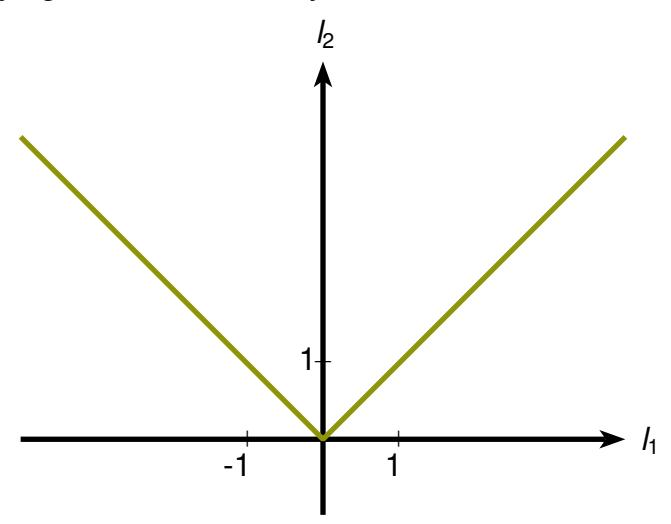
\includegraphics[width=0.5\textwidth]{img/_page_119_Figure_6.jpeg}
\end{center}
Gráfico de $f(x)=|x|$.

\subsection*{Ejemplo 4: función definida por tramos (a partir de circunferencias)}

Graficar
\[
f(x) = \begin{cases} \sqrt{1-x^2} & \text{si } x \ge 0, \\
\sqrt{1-\dfrac{x^2}{9}} & \text{si } x < 0. \end{cases}
\]

Para $x \ge 0$: $y=f(x) \leftrightarrow y=\sqrt{1-x^2} \leftrightarrow y \ge 0 \land x^2+y^2=1$.
Como $x^2+y^2=1$ es una circunferencia de radio $1$, y exigimos además $x\ge0$, $y\ge0$, obtenemos
el arco de esa circunferencia ubicado en el primer cuadrante, entre $(1,0)$ y $(0,1)$.

Para $x<0$: $y=f(x) \leftrightarrow y \ge 0 \land \dfrac{x^2}{9}+y^2=1$, que corresponde a una
elipse; junto con $x<0$, $y\ge0$, se obtiene el arco de esa elipse en el segundo cuadrante, entre
$(-3,0)$ y $(0,1)$.

\begin{center}
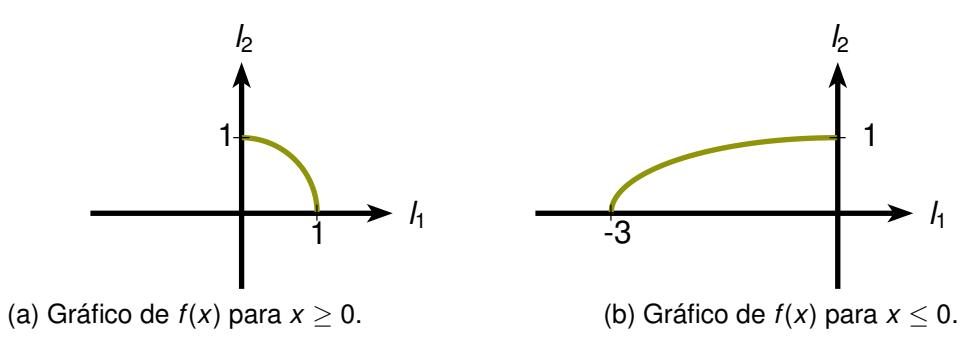
\includegraphics[width=0.85\textwidth]{img/_page_120_Figure_7.jpeg}
\end{center}
Gráfico de $f(x)$ en cada región por separado.

Uniendo ambos tramos (que coinciden en $x=0$, donde ambos dan $y=1$) se obtiene el gráfico completo
de $f$:

\begin{center}
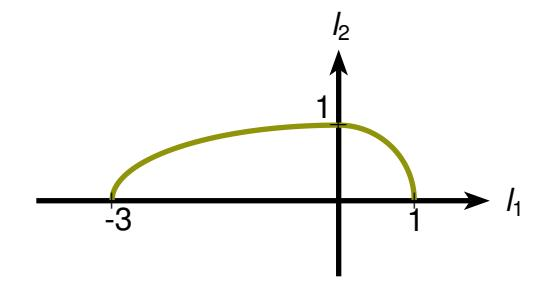
\includegraphics[width=0.5\textwidth]{img/_page_120_Figure_10.jpeg}
\end{center}
Gráfico de $f(x)$.

\end{document}
